\chapter{2015年2、3月份间的宇宙线测试数据分析}

\section{触发时间间隔分布}
\subsection{问题描述}
一般认为宇宙线事例的时间间隔分布满足指数衰减规律,即
\begin{equation}
	P(t) = \frac{1}{T_{interval}}e^{-t/T_{interval}}
\end{equation}
其中,$T_{interval}$是宇宙线事例的平均时间间隔。

\subsection{结果}
对test21文件进行分析得到如下典型结果。这些结果无论是对MWDC板的Bunch ID,还是对TOF板的Bunch ID或Leading Time都是一致的。

\subsubsection*{事件发生的时间戳在测量时间范围内呈均匀分布}
MWDC板和TOF板的Bunch ID在$[0,4095]$呈均匀分布,TOF板的Leading Time在$[0,2097151]$呈均匀分布,典型示例如图\ref{fig:tof_leadingtime_distribution}所示。
\begin{figure}[htbp]
	\centering
	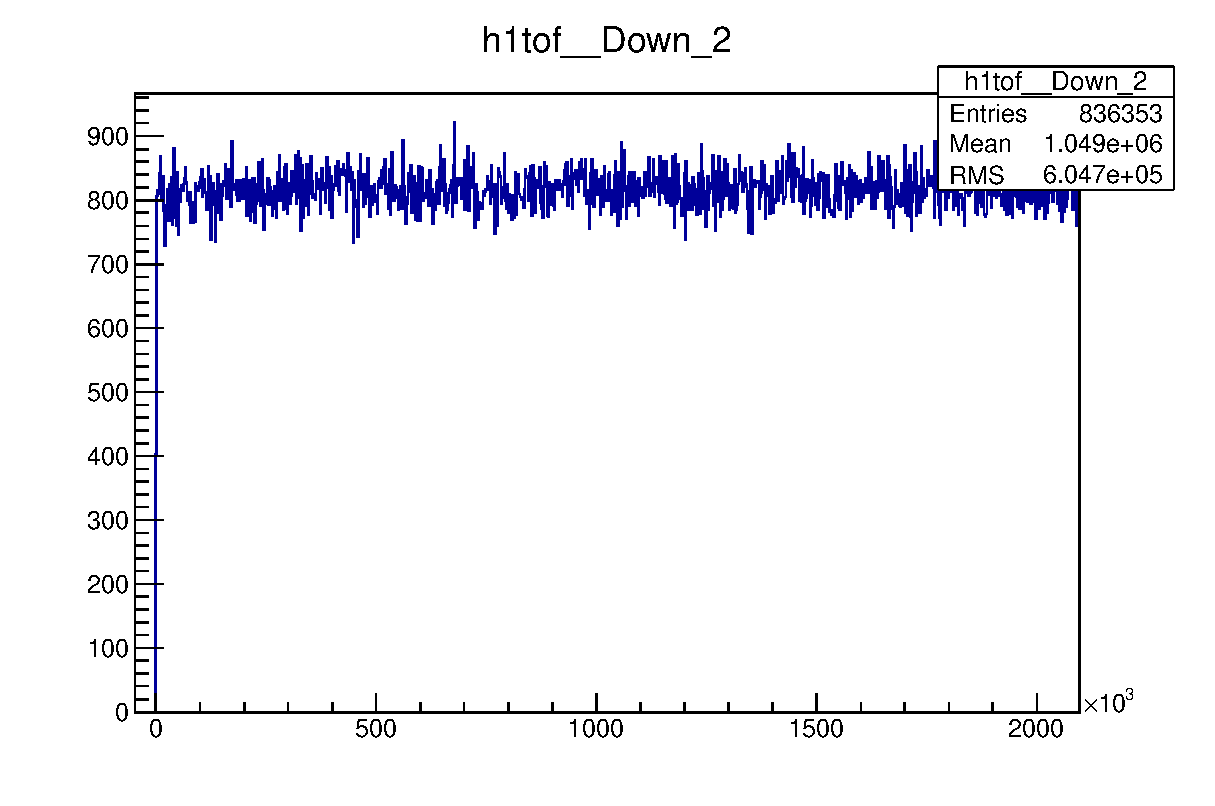
\includegraphics[width=0.95\textwidth]{fig/tof_leadingtime_distribution.eps}
	\caption{TOF板测得的Leading Time原始分布}
	\label{fig:tof_leadingtime_distribution}
\end{figure}

\subsubsection*{前后两个事件的时间戳关联呈统计无关}
MWDC板和TOF板的前后事件间的Bunch ID关联,以及TOF板的Leading Time关联呈统计无关,典型示例如图\ref{fig:tof_leadingtime_current_vs_previous}所示。
\begin{figure}[H]
	\centering
	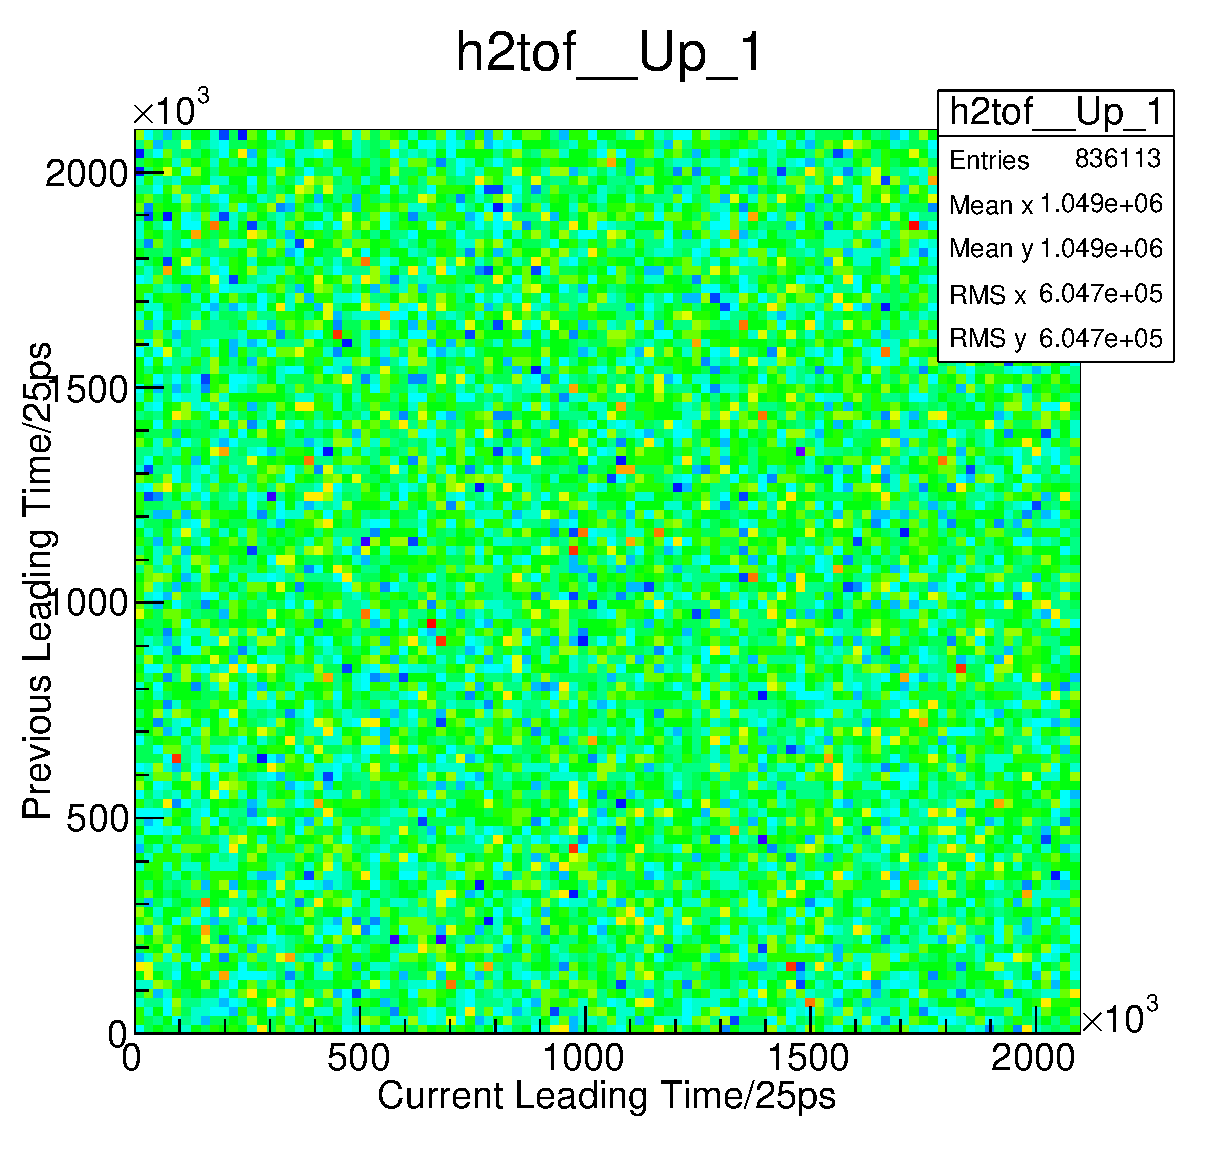
\includegraphics[width=0.8\textwidth]{fig/tof_leadingtime_current_vs_previous.eps}
	\caption{TOF板测得的相邻事件Leading Time的关联性}
	\label{fig:tof_leadingtime_current_vs_previous}
\end{figure}
此结果需要思考,因为实际中,宇宙线事例的时间间隔分布是有一定概率分布的,满足指数衰减规律。而测量结果确模糊了这种关联性。

\subsubsection*{触发时间间隔呈等腰三角形分布}
将前后事件的时间戳(Bunch ID或Leading Time)直接相减得到的触发时间分布呈等腰三角形.
图\ref{fig:bunchid_interval}给出了MWDC和TOF板得到的Bunch ID时间间隔分布。
\begin{figure}[htbp]
	\centering
	\begin{subfigure}[b]{0.48\textwidth}
        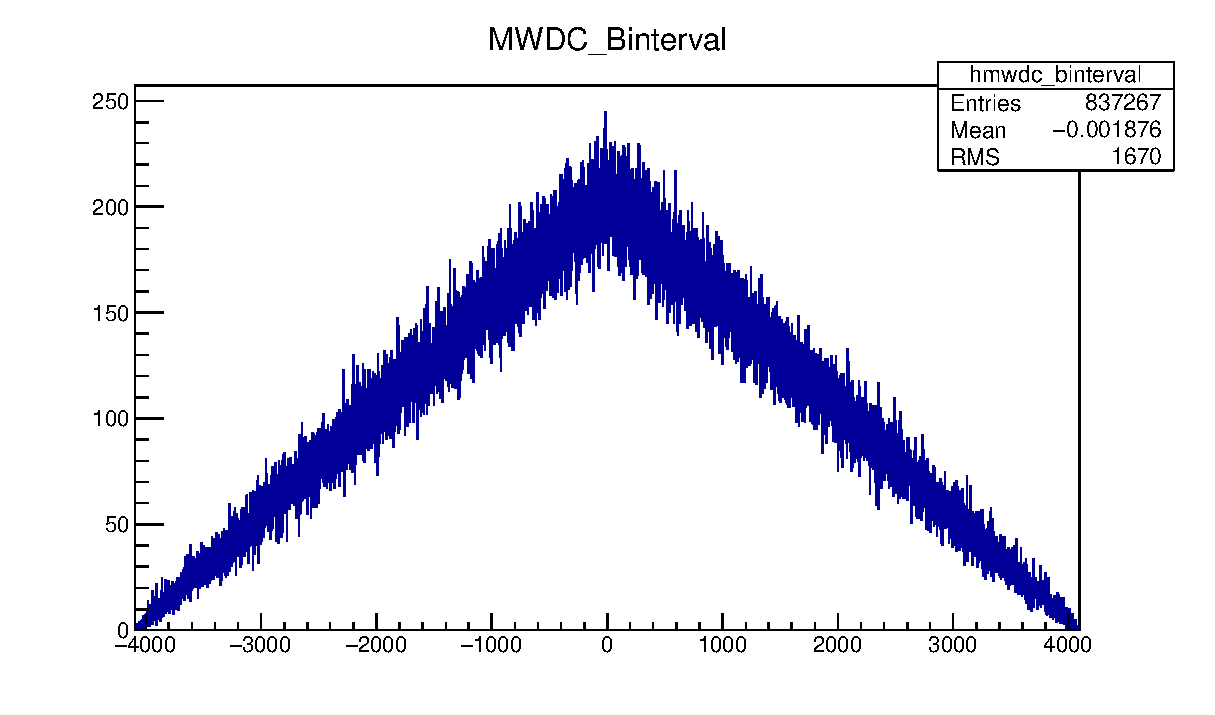
\includegraphics[width=\textwidth]{fig/mwdc_bunchid_interval.eps}
        \caption{MWDC}
        \label{fig:mwdc_bunchid_interval}
    \end{subfigure}
    ~
    \begin{subfigure}[b]{0.48\textwidth}
        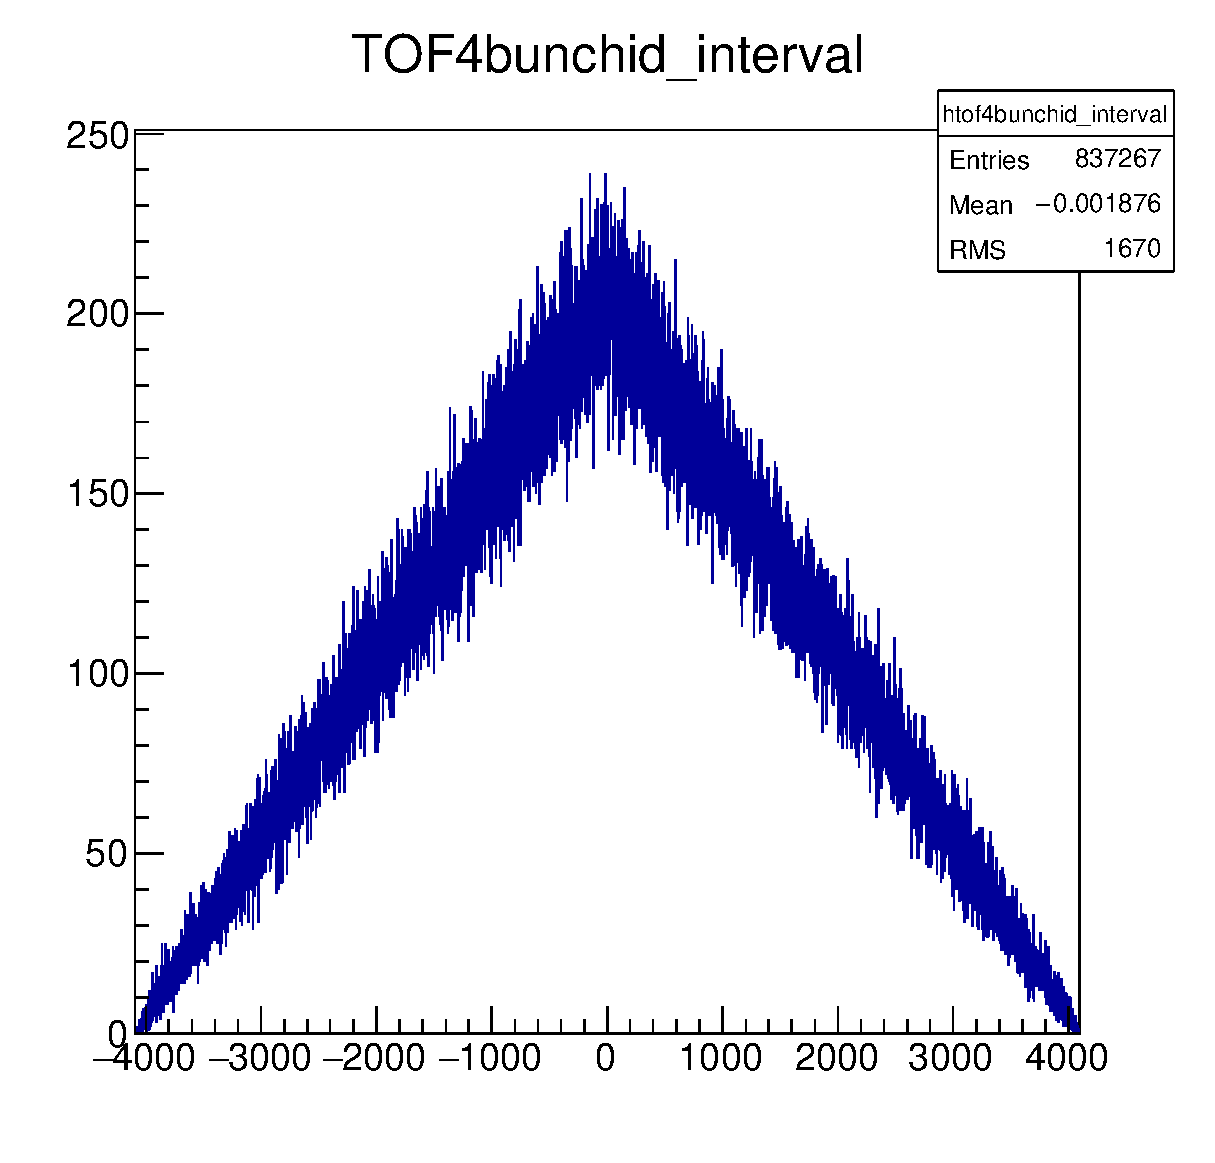
\includegraphics[width=\textwidth]{fig/tof_bunchid_interval.eps}
        \caption{TOF}
        \label{fig:tof_bunchid_interval}
    \end{subfigure}
	\caption{Bunch ID的时间间隔分布}
	\label{fig:bunchid_interval}
\end{figure}

若对时间测量的roll over进行修正,则得到的时间间隔分布在测量范围内是均匀的,如图\ref{fig:tof_interval_rollover}所示。
roll over修正是指:由于时间测量范围有限,时间戳在一定周期后会自动翻转再从0开始,此时后一事件的时间戳可能小于前一事件的时间戳,此时将后一事件的时间戳测量值加上时间测量量程后再进行相减。
\begin{figure}[htbp]
	\centering
	\begin{subfigure}[b]{0.48\textwidth}
        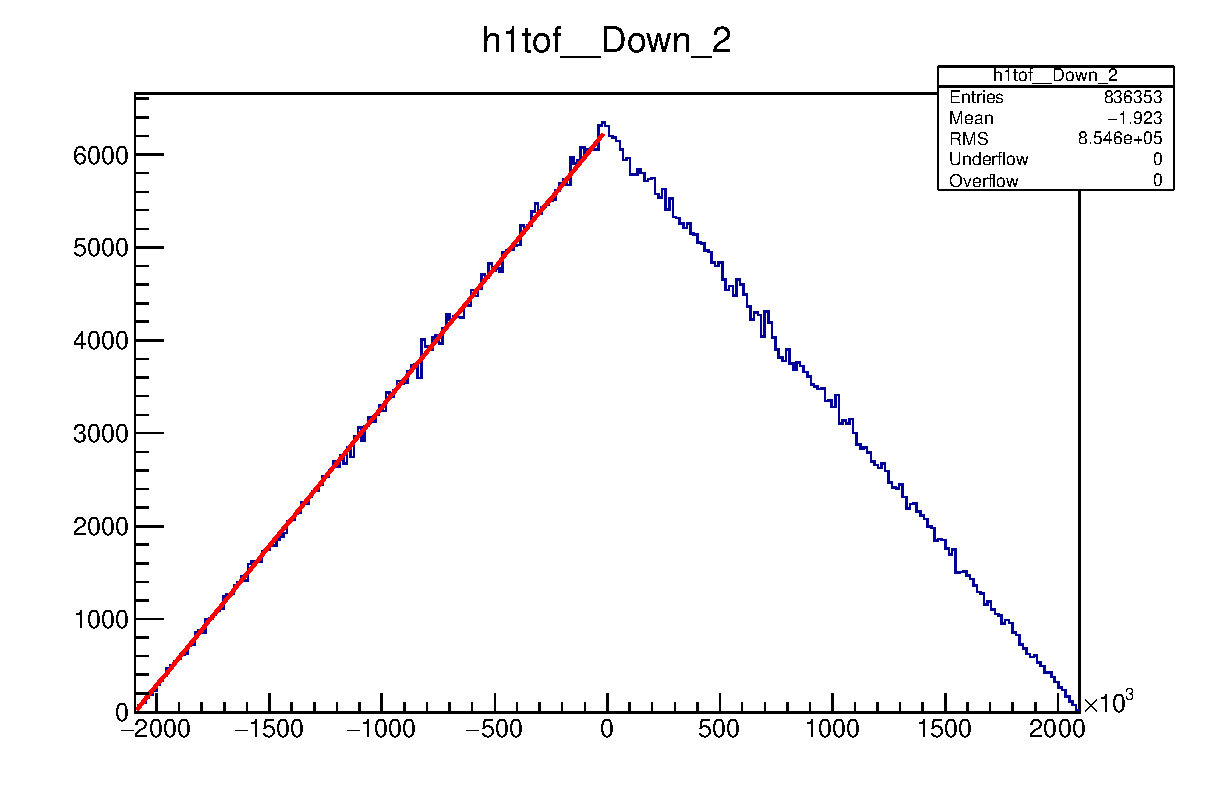
\includegraphics[width=\textwidth]{fig/tof_interval.eps}
        \caption{roll over修正前}
        \label{fig:tof_interval}
    \end{subfigure}
~
    \begin{subfigure}[b]{0.48\textwidth}
        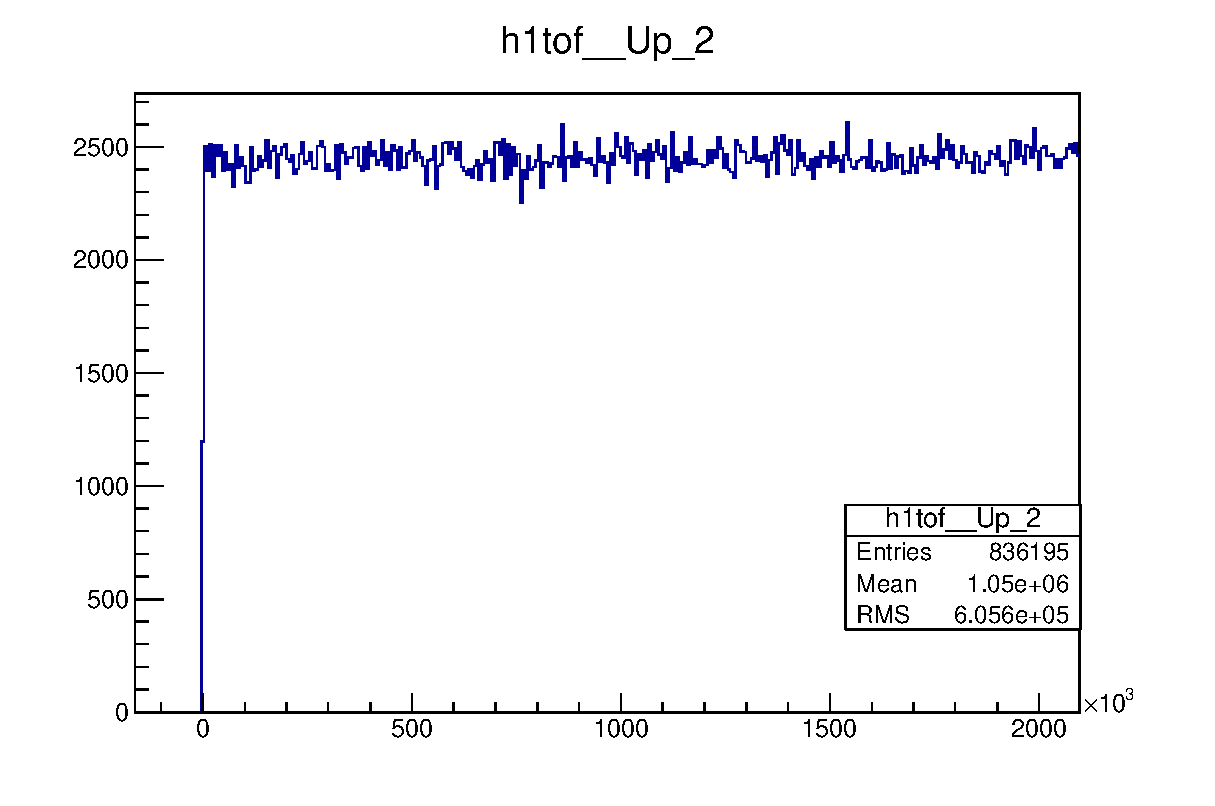
\includegraphics[width=\textwidth]{fig/tof_interval_correct_rollover.eps}
        \caption{roll over修正后}
        \label{fig:tof_interval_correct_rollover}
    \end{subfigure}
	\caption{TOF板得到的Leading Time时间间隔分布在roll over进行修正前后}
	\label{fig:tof_interval_rollover}
\end{figure}

\subsection{讨论}
等腰三角形分布可以用两种方法进行解释:
\subsubsection*{从指数衰减分布出发}
条件:时间间隔$T_{interval}$满足指数衰减分布,时间常数为$\lambda$,且时间测量量程$R\ll\lambda$。在测量量程内的时间戳为$T_{measusred}=T_{real}\mod R$,其中$T_{real}$是实际的时间间隔大小。

根据上述条件可以得到:
\begin{align}
&\begin{cases}
dT_{measured} =dT_{real}\\
\frac{P}{P+dP} = \frac{\sum\limits_{n=0}^{\infty}e^{-(T_{measured}+nR)/\lambda}}{\sum\limits_{n=0}^{\infty}e^{-(T_{measured}+dT_{measured}+nR)/\lambda}}
\end{cases}\\
\Rightarrow &\frac{dP}{P}=-\frac{dT_{measured}}{\lambda}\\
\Rightarrow &P(T_{measured})\propto e^{-\frac{T_{measured}}{\lambda}}, T_{measured}\in[0,R]
\end{align}

进一步考虑roll over对概率分布的影响。
由于时间戳在量程范围内是均匀分布的,因此对于某一确定的$T_{measured}$,其时间间隔为正值所占的比例应该是$\frac{R-T_{measured}}{R}$,为负值的比例应该是$\frac{T_{measured}}{R}$。
由此可以得到,不考虑roll over修正的概率分布为
\begin{equation}
	\begin{cases}
	P(T_{measured})=\frac{R-T_{measured}}{R}e^{-\frac{T_{measured}}{\lambda}} & ,T_{measured}\in[0,R]\\
	P(T_{measured})=\frac{R+T_{measured}}{R}e^{-\frac{T_{measured}+R}{\lambda}} &,T_{measured}\in[-R,0]\\
	\end{cases}
\end{equation}

上式在$R\ll\lambda$时,就是等腰三角形分布,如图\ref{fig:interval_pdf}所示
\begin{figure}[htbp]
	\centering
	\begin{subfigure}[b]{0.48\textwidth}
        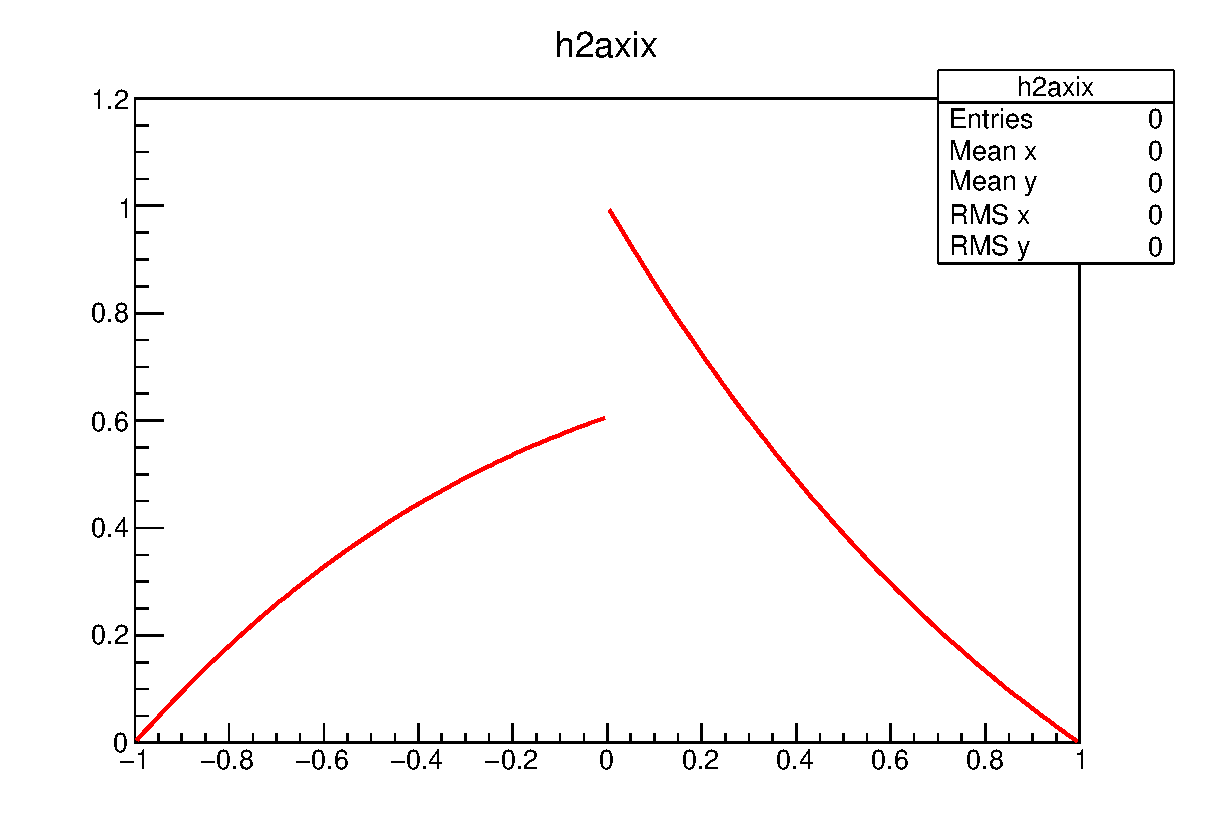
\includegraphics[width=\textwidth]{fig/interval_pdf_largerange.eps}
        \caption{$R\simeq\lambda$}
    \end{subfigure}
    \begin{subfigure}[b]{0.48\textwidth}
        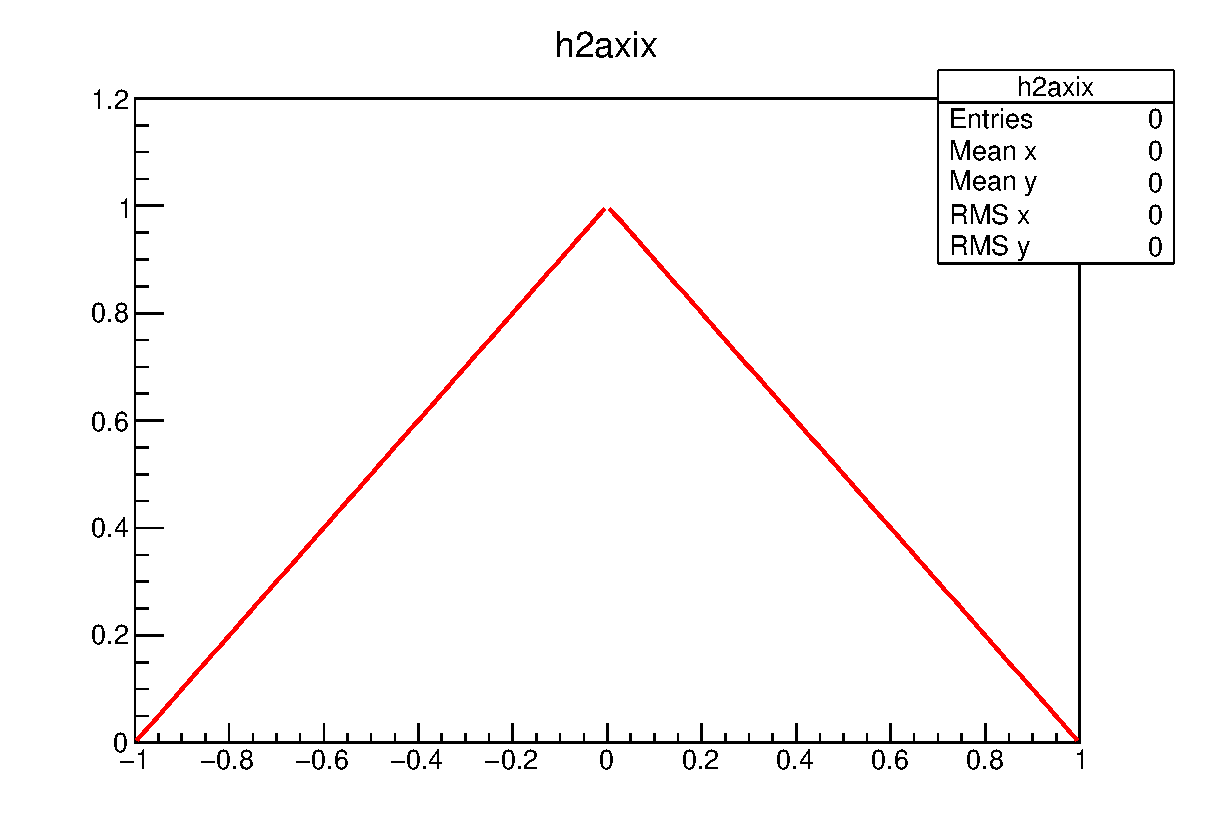
\includegraphics[width=\textwidth]{fig/interval_pdf_smallrange.eps}
        \caption{$R\ll\lambda$}
    \end{subfigure}
	\caption{测量范围从大到小的演化}
	\label{fig:interval_pdf}
\end{figure}


\subsubsection*{从均匀随机分布出发}
由上述结果中得到前后事件的时间戳分别呈均匀分布,且相互独立(无统计关联)。
假设$T_{current}$和$T_{previous}$分布是前后事件的时间戳,它们的取值范围为$[0,R]$,其中R是时间测量量程,而${T_interval=T_{current}+(-T_{previous})}$。令$Z=T_{interval}$,$Y=T_{current}$,$X=-T_{previous}$,则$Z=Y+X$,即随机变量$Z$是两个相互独立的随机变量$X、Y$之和,其中
\begin{align}
P(Y)&=1, Y\in [0,R]\\
P(X)&=1, X\in [-R,0]
\end{align}
两个独立随机变量之和的概率分布是这两个分布的卷积。且对于均匀分布的随机变量来说,其和的概率分布,通过卷积公式计算得到的就是等腰三角形分布,即
\begin{equation}
	\begin{cases}
	P(Z)=Z+R,&(-R\leq Z \leq 0)\\
	P(Z)=R-Z,&(0\leq Z \leq R)
	\end{cases}
\end{equation}

\subsection{遗留问题}
\underline{上述两种解释是否可以统一?}

\section{TOF获取卡Bunch ID与Leading Time之差}
四块TOF获取卡的Bunch ID与Leading Time之间的差值基本都稳定在$10*25=250ns$左右。

\begin{figure}[htbp]
	\centering
	\begin{subfigure}[b]{0.48\textwidth}
        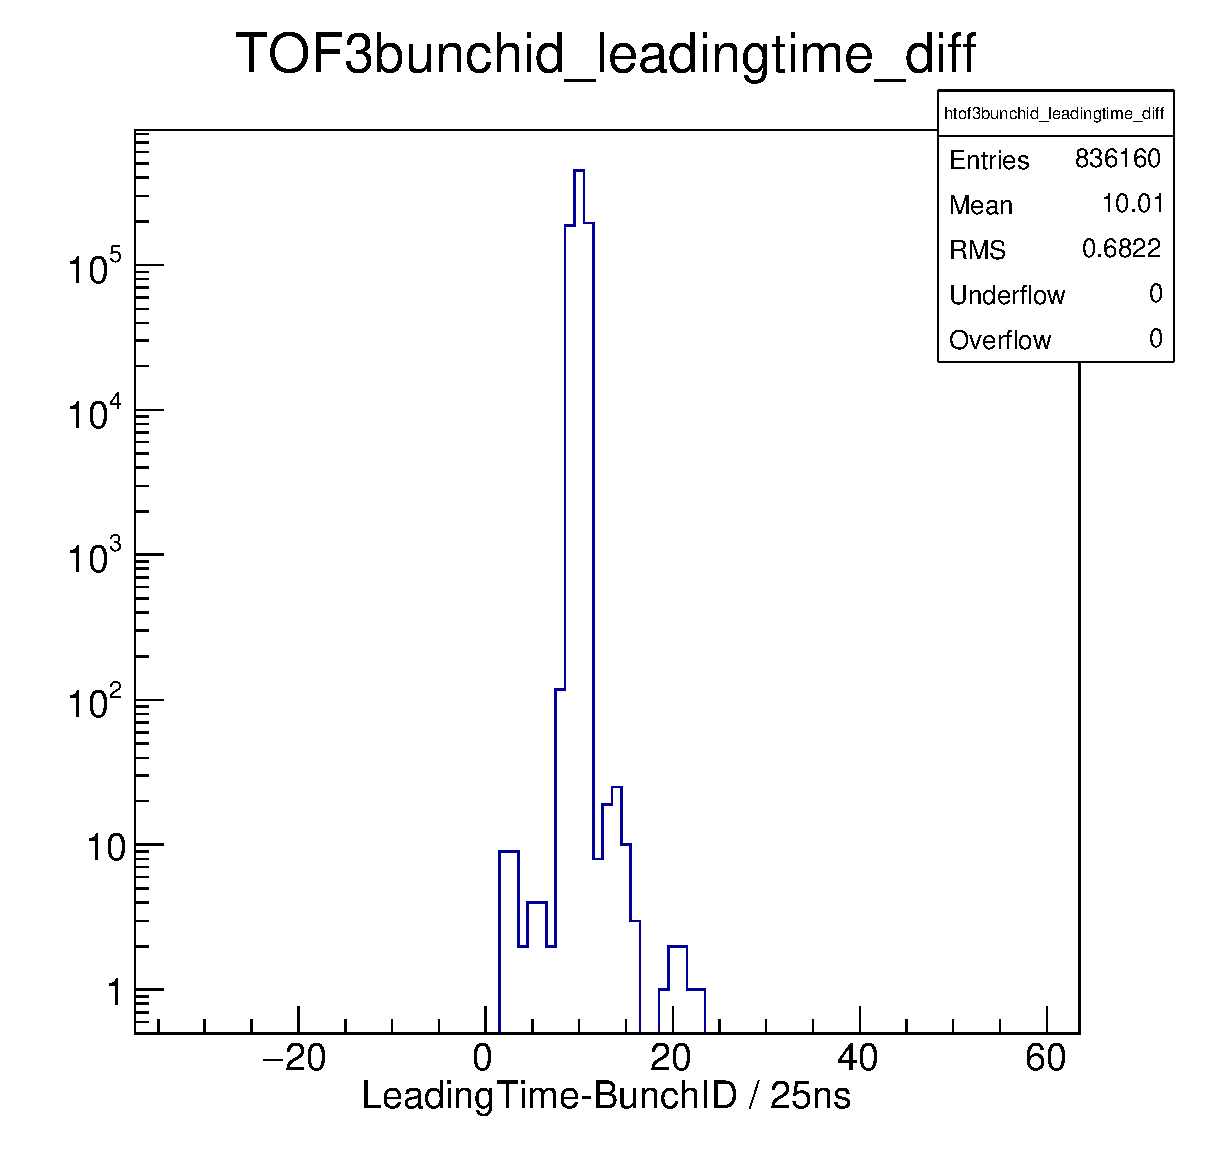
\includegraphics[width=\textwidth]{fig/tof_leadingtime_bunchid_diff.eps}
        \caption{TOF板Leading Time与Bunch ID之差的典型分布}
    \end{subfigure}
    \begin{subfigure}[b]{0.48\textwidth}
        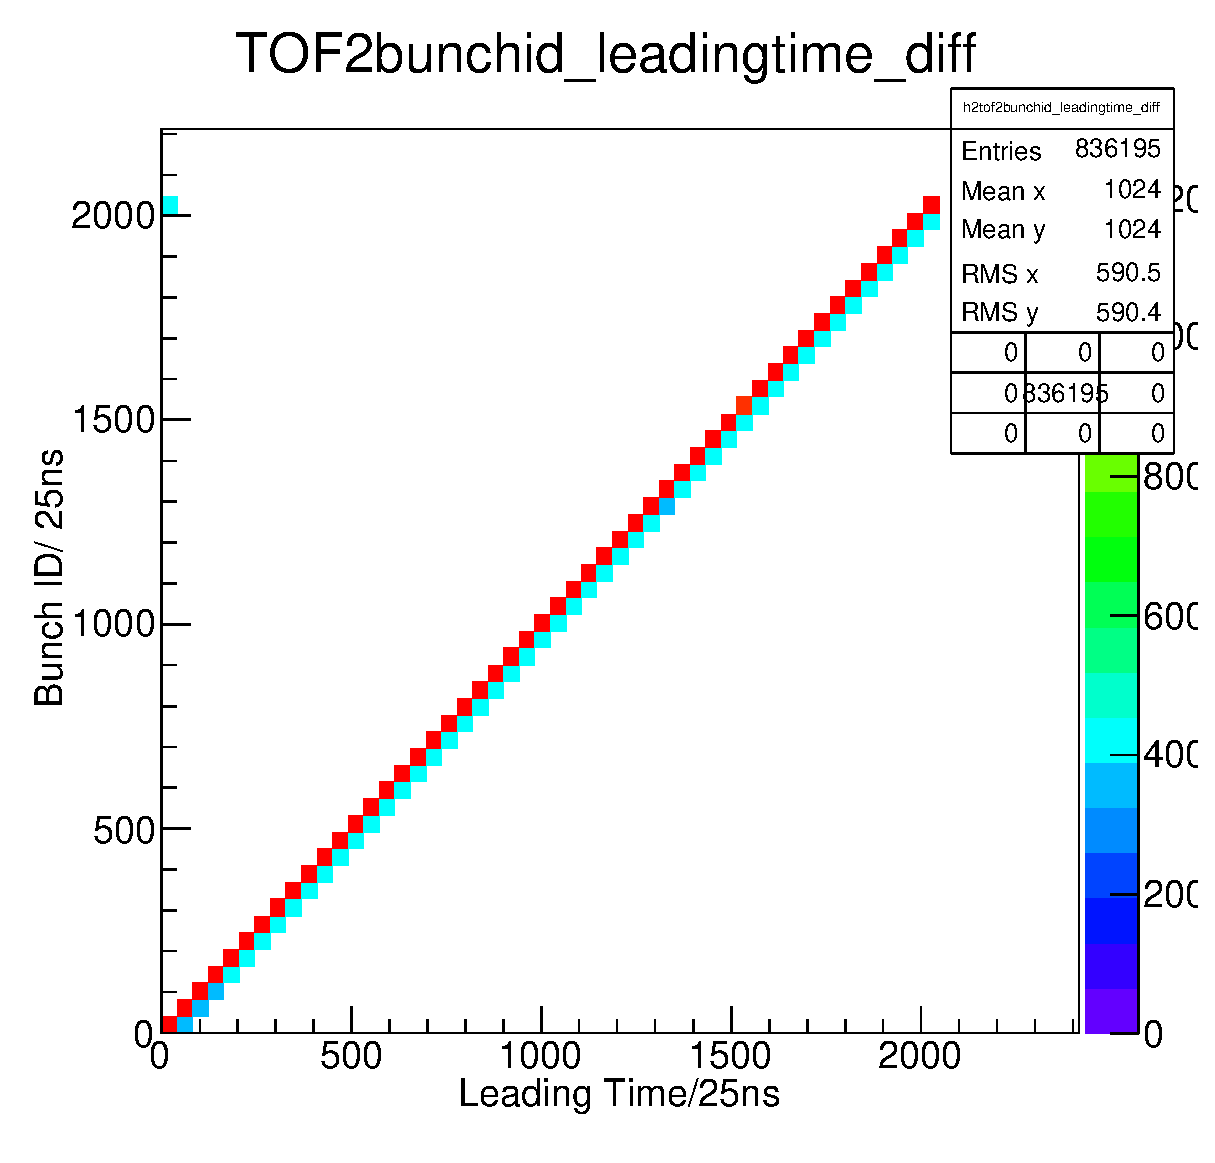
\includegraphics[width=\textwidth]{fig/tof_leadingtime_vs_bunchid.eps}
        \caption{TOF板Leading Time与Bunch ID的关联图}
    \end{subfigure}
	\caption{Leading Time与Bunch ID的关系}
	\label{fig:tof_leadingtime_bunchid}
\end{figure}

\section{获取卡间的时间同步(Time and event synchronization among different DAQ cards)}
\subsection{结果}
\subsubsection*{Event ID}
每块获取卡的Event ID是连续的,没有出现丢事件的情况。
大部分获取卡的起始Event ID为零,但偶尔会出现不为零的情况。此时,获取卡间的事件应该仍然是同步的。

\subsubsection*{Bunch ID}

\section{TOF板的无信号通道数}

\section{单通道的多击中数(Multi-hits in a single channel)}

\section{MWDC单个丝面的击中多重数(Multiplicity in a single MWDC wireplane}